\section{Results}

A plot of the magnetic field from the earth is shown in figure \ref{fig:earth} with the dimensionless length scales on the axes. 

\begin{figure}[htb]
	\centering
	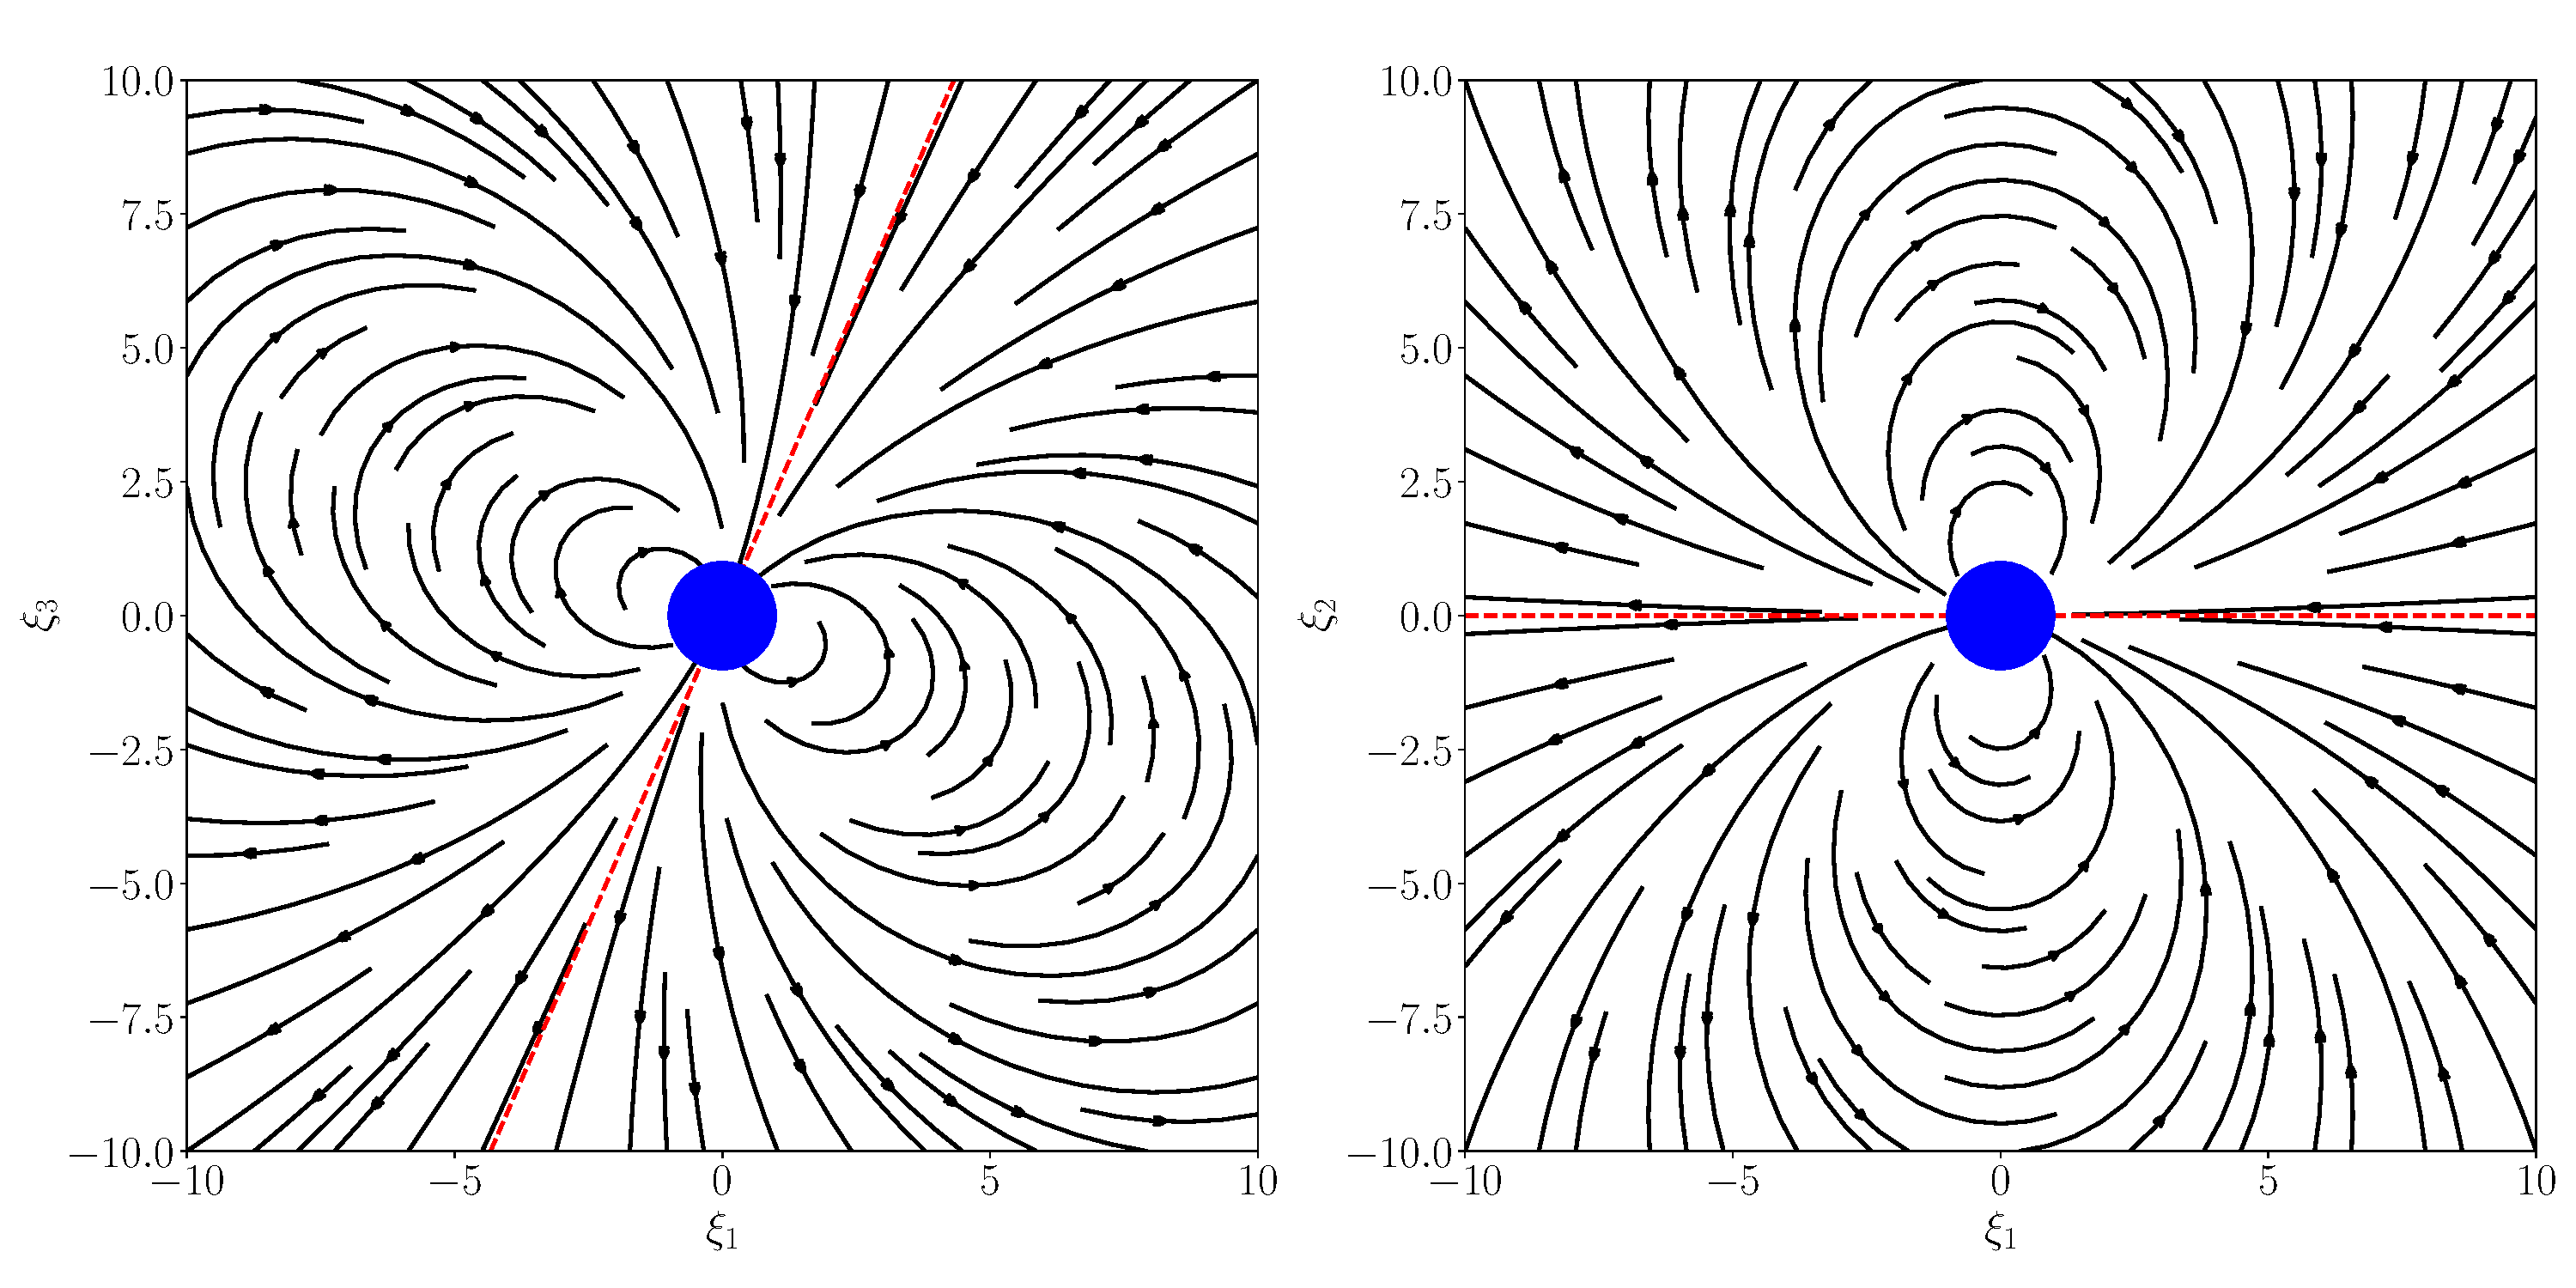
\includegraphics[width=\columnwidth]{../fig/earth.pdf}
	\caption{Magnetic field from earth.}
	\label{fig:earth}
\end{figure}

When sending particles far from the earth towards it they start oscillating around the field lines as they approach the earth. This is consistent with the more familiar and simple case of Larmor precession in a uniform field. This is shown in figure \ref{fig:fast_part} and \ref{fig:slow_part}. Also apparent from these plots is that the radius of precession is larger when the particles are sent towards the earth with larger speed.

\begin{figure}[htb]
	\centering
	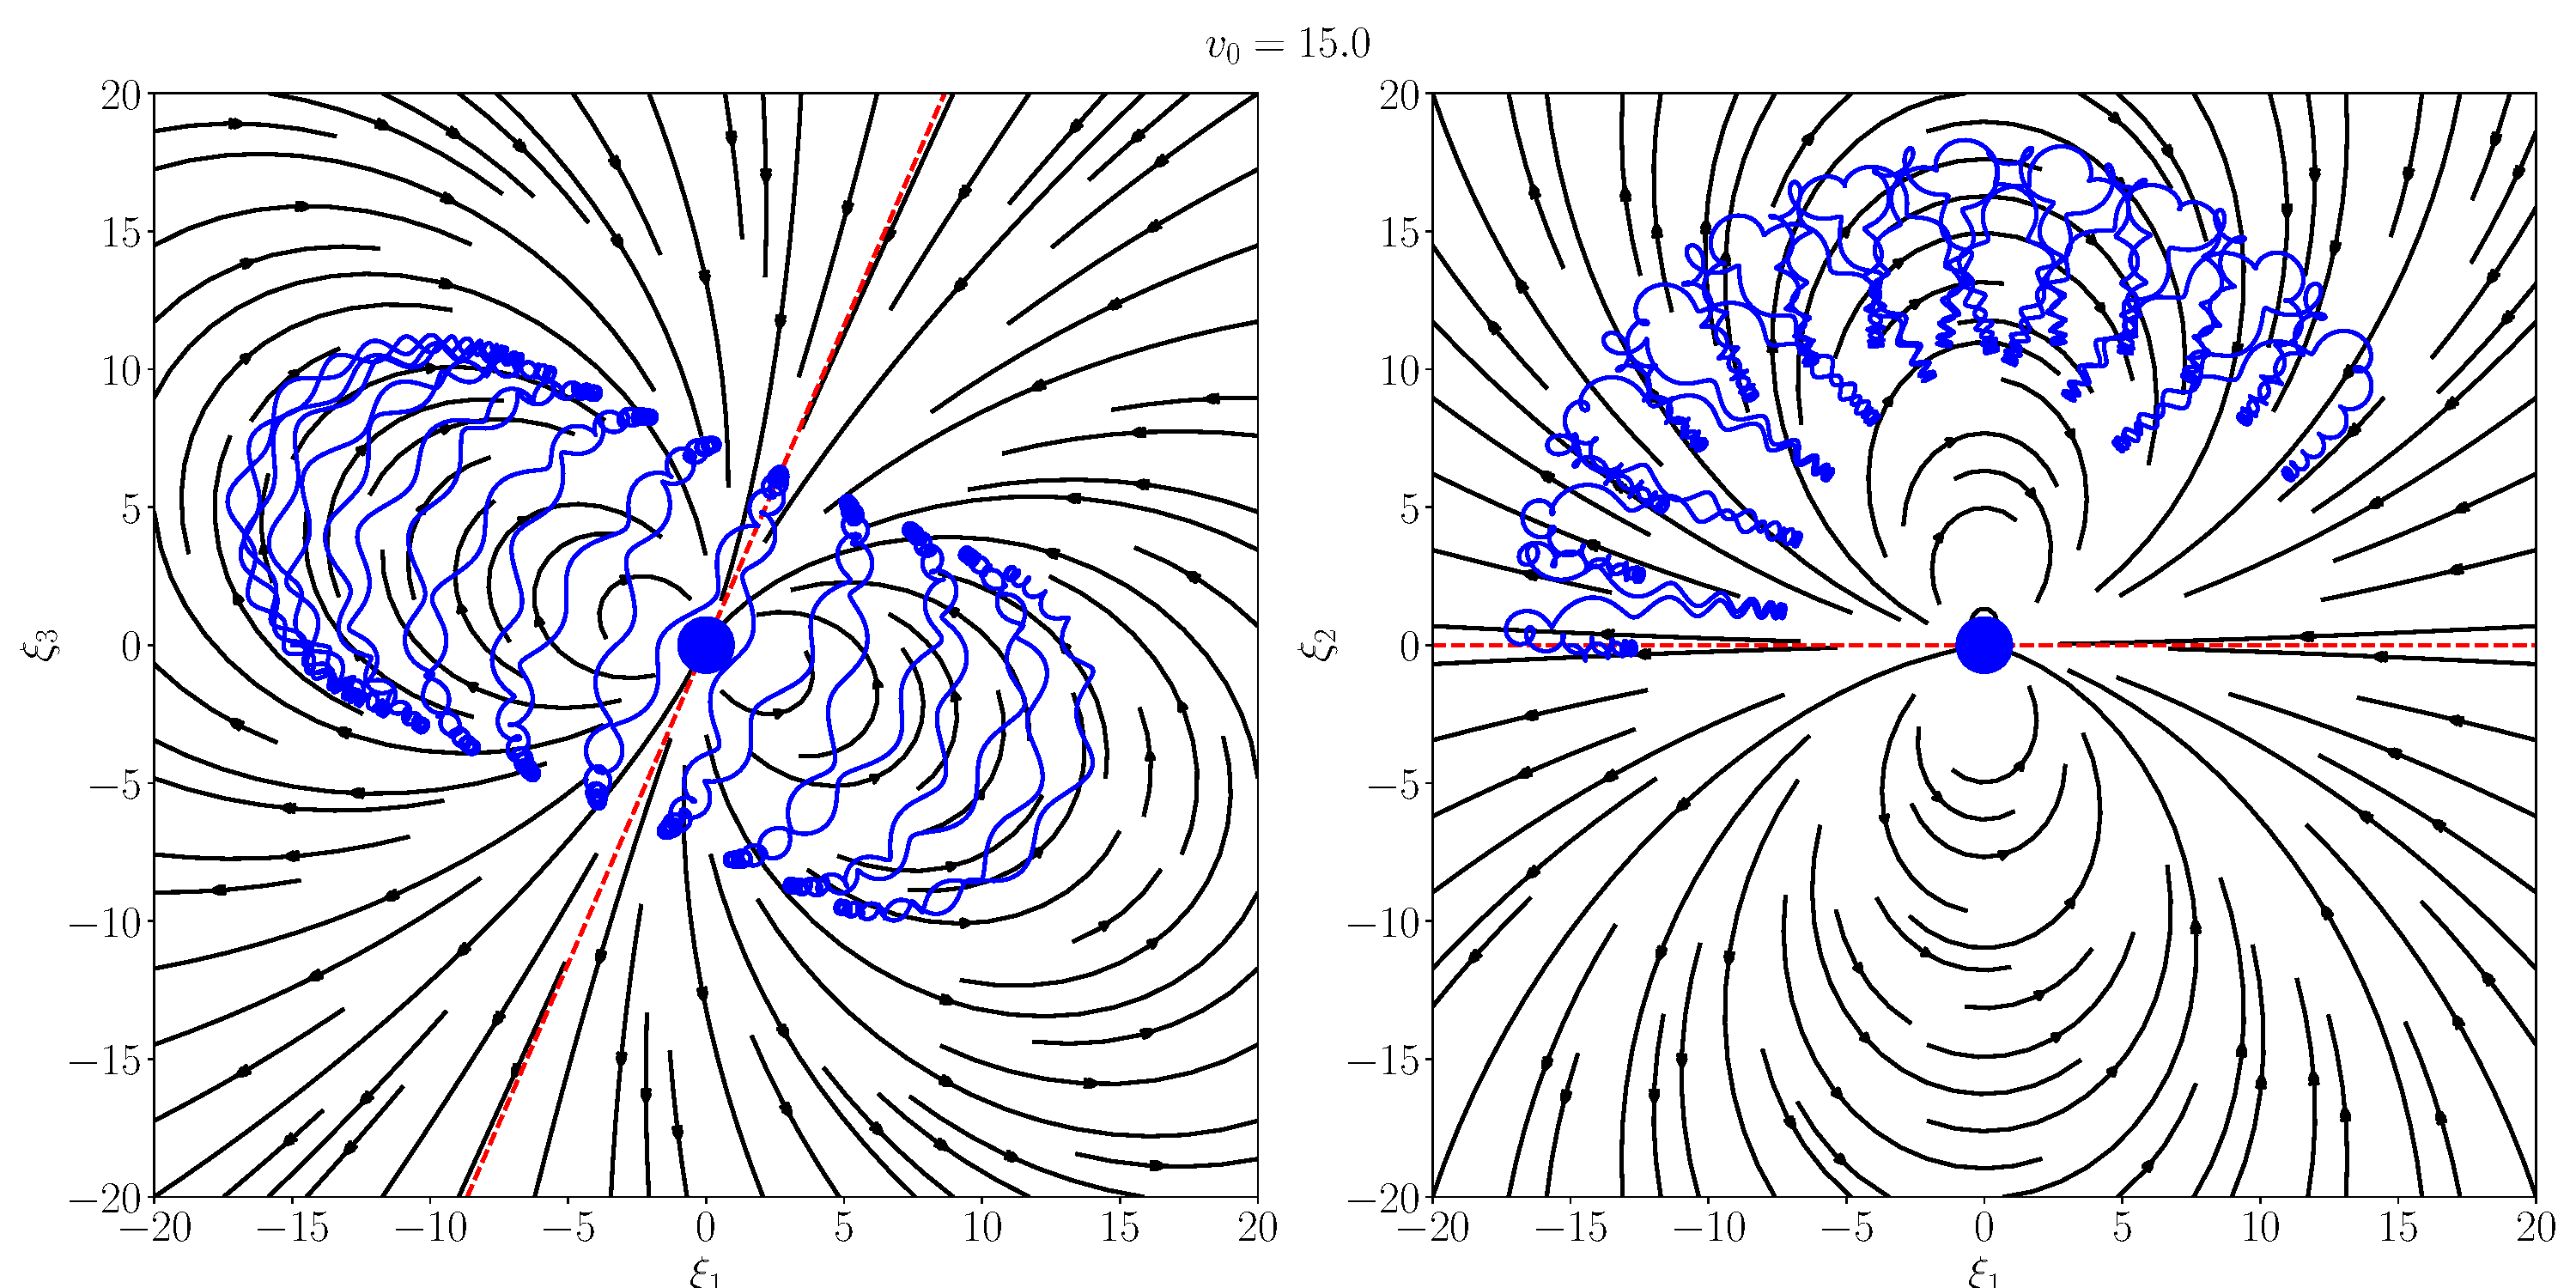
\includegraphics[width=\columnwidth]{../fig/earth_traj_fast.pdf}
	\caption{Particle sent towards the earth with typical solar wind velocity.}
	\label{fig:fast_part}
\end{figure}

The trajectories of particles sent towards earth at different heights $z$ ($\xi_3$) is shown in figure \ref{fig:different_z}.

\begin{figure}[htb]
	\centering
	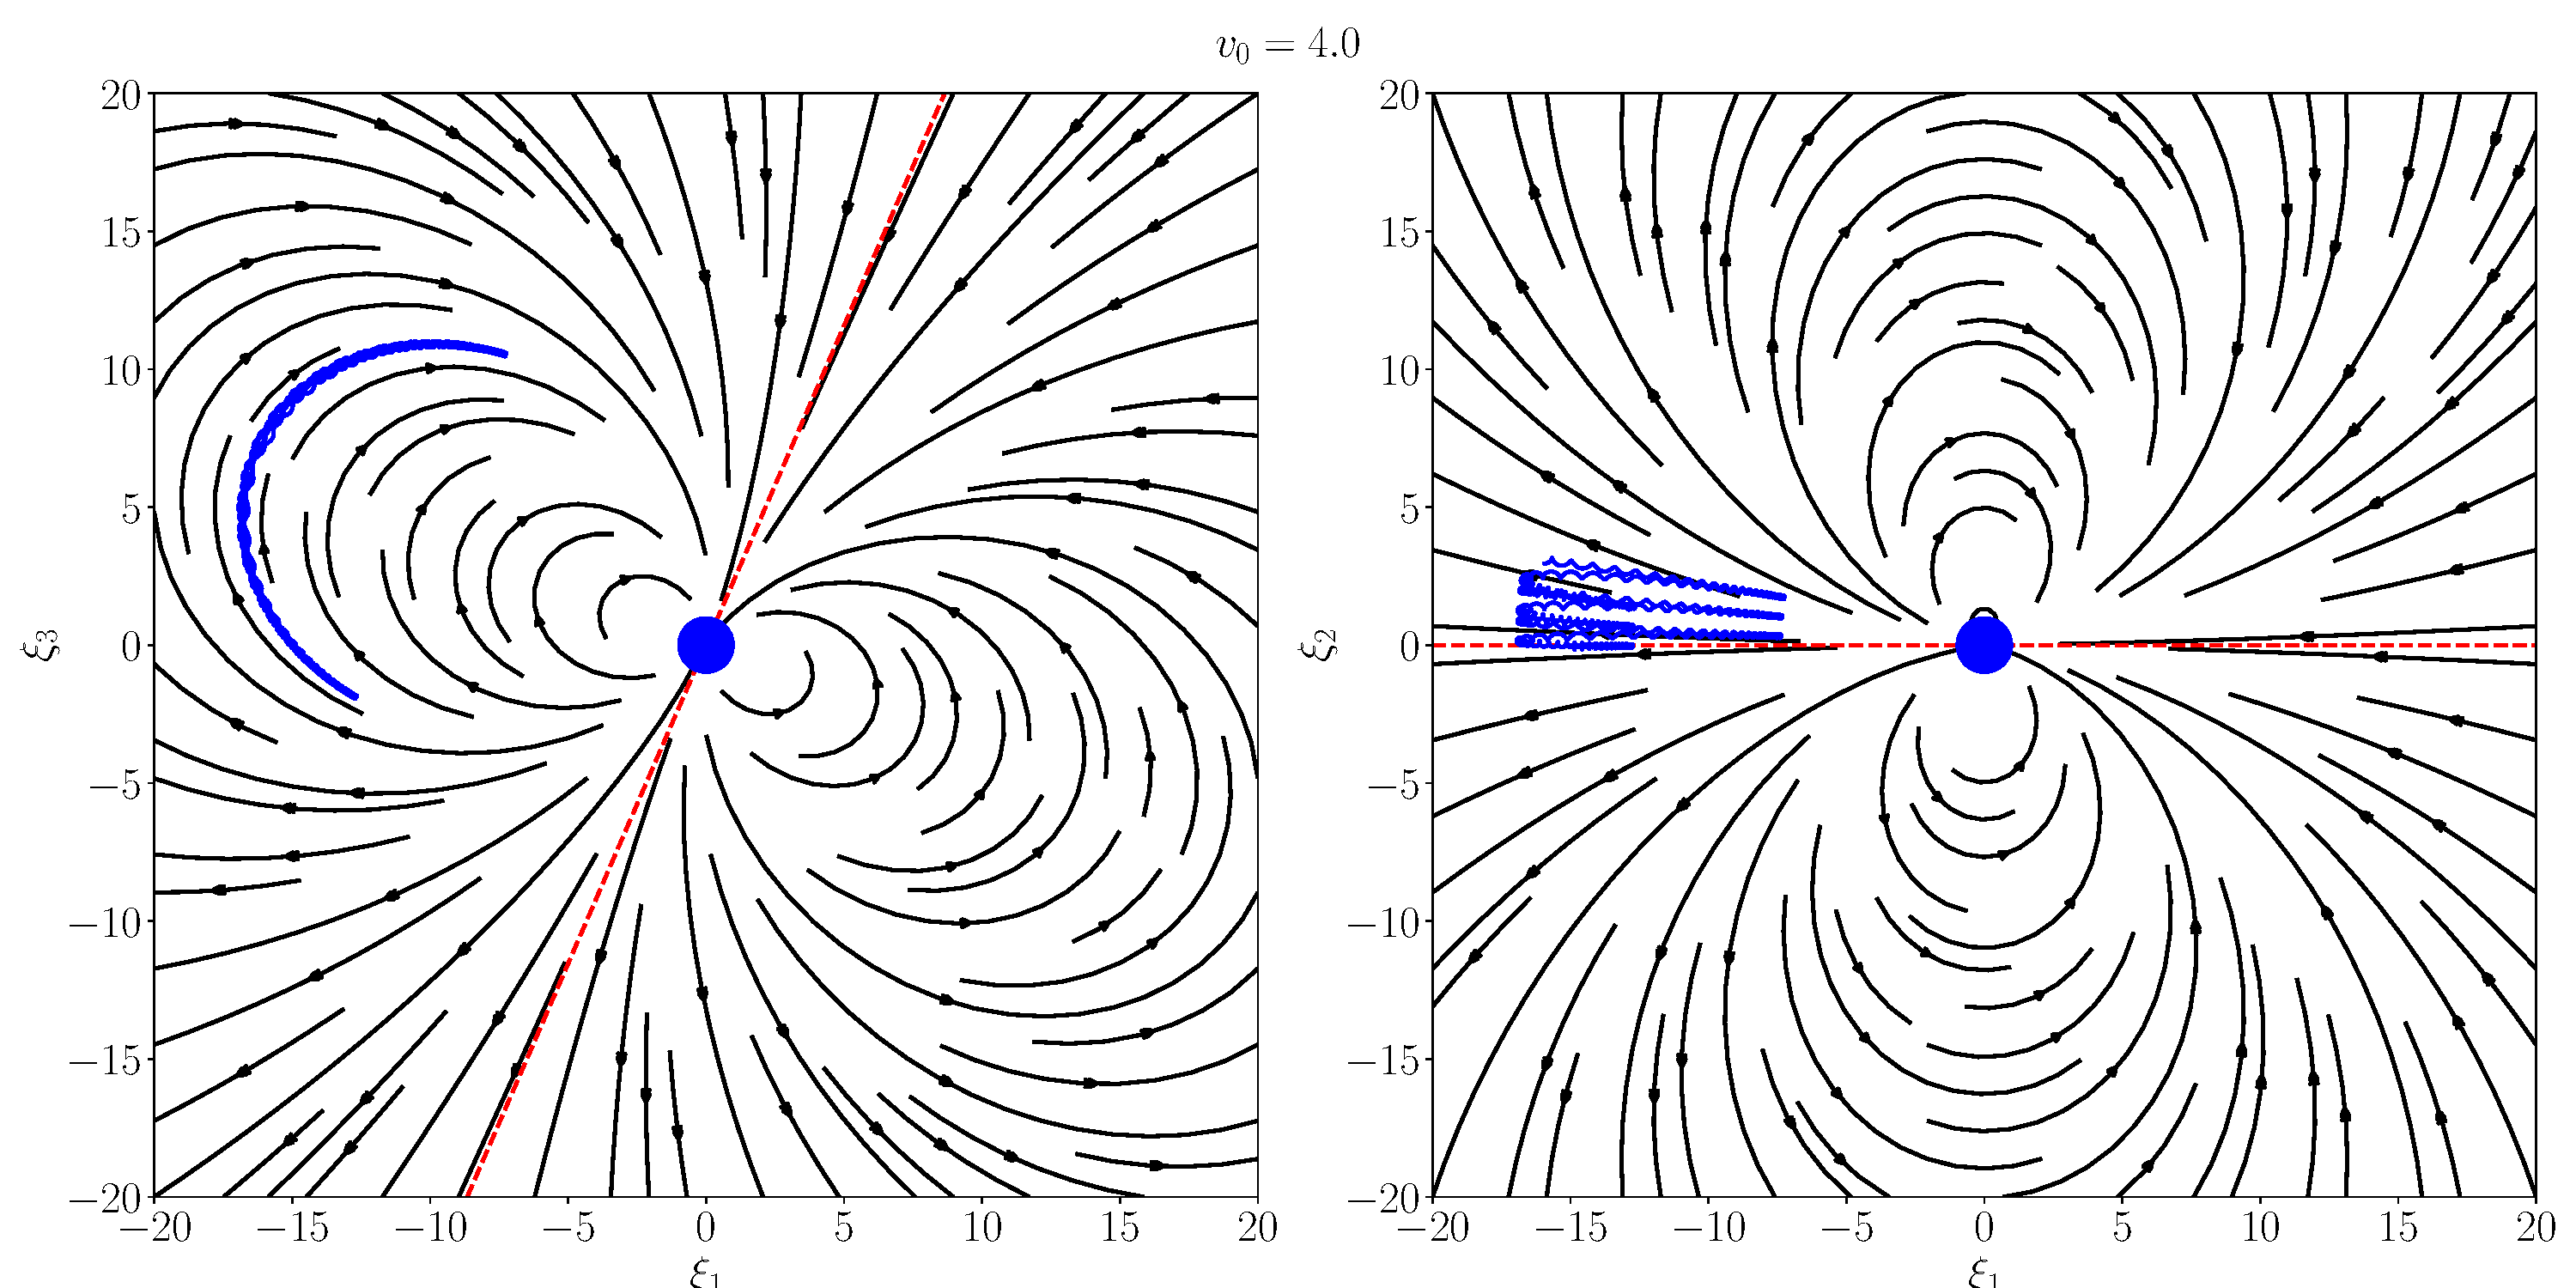
\includegraphics[width=\columnwidth]{../fig/earth_traj_slow.pdf}
	\caption{Particle sent towards the earth with lower typical solar wind velocity.}
	\label{fig:slow_part}
\end{figure}
\begin{figure}[h!]
	\centering
	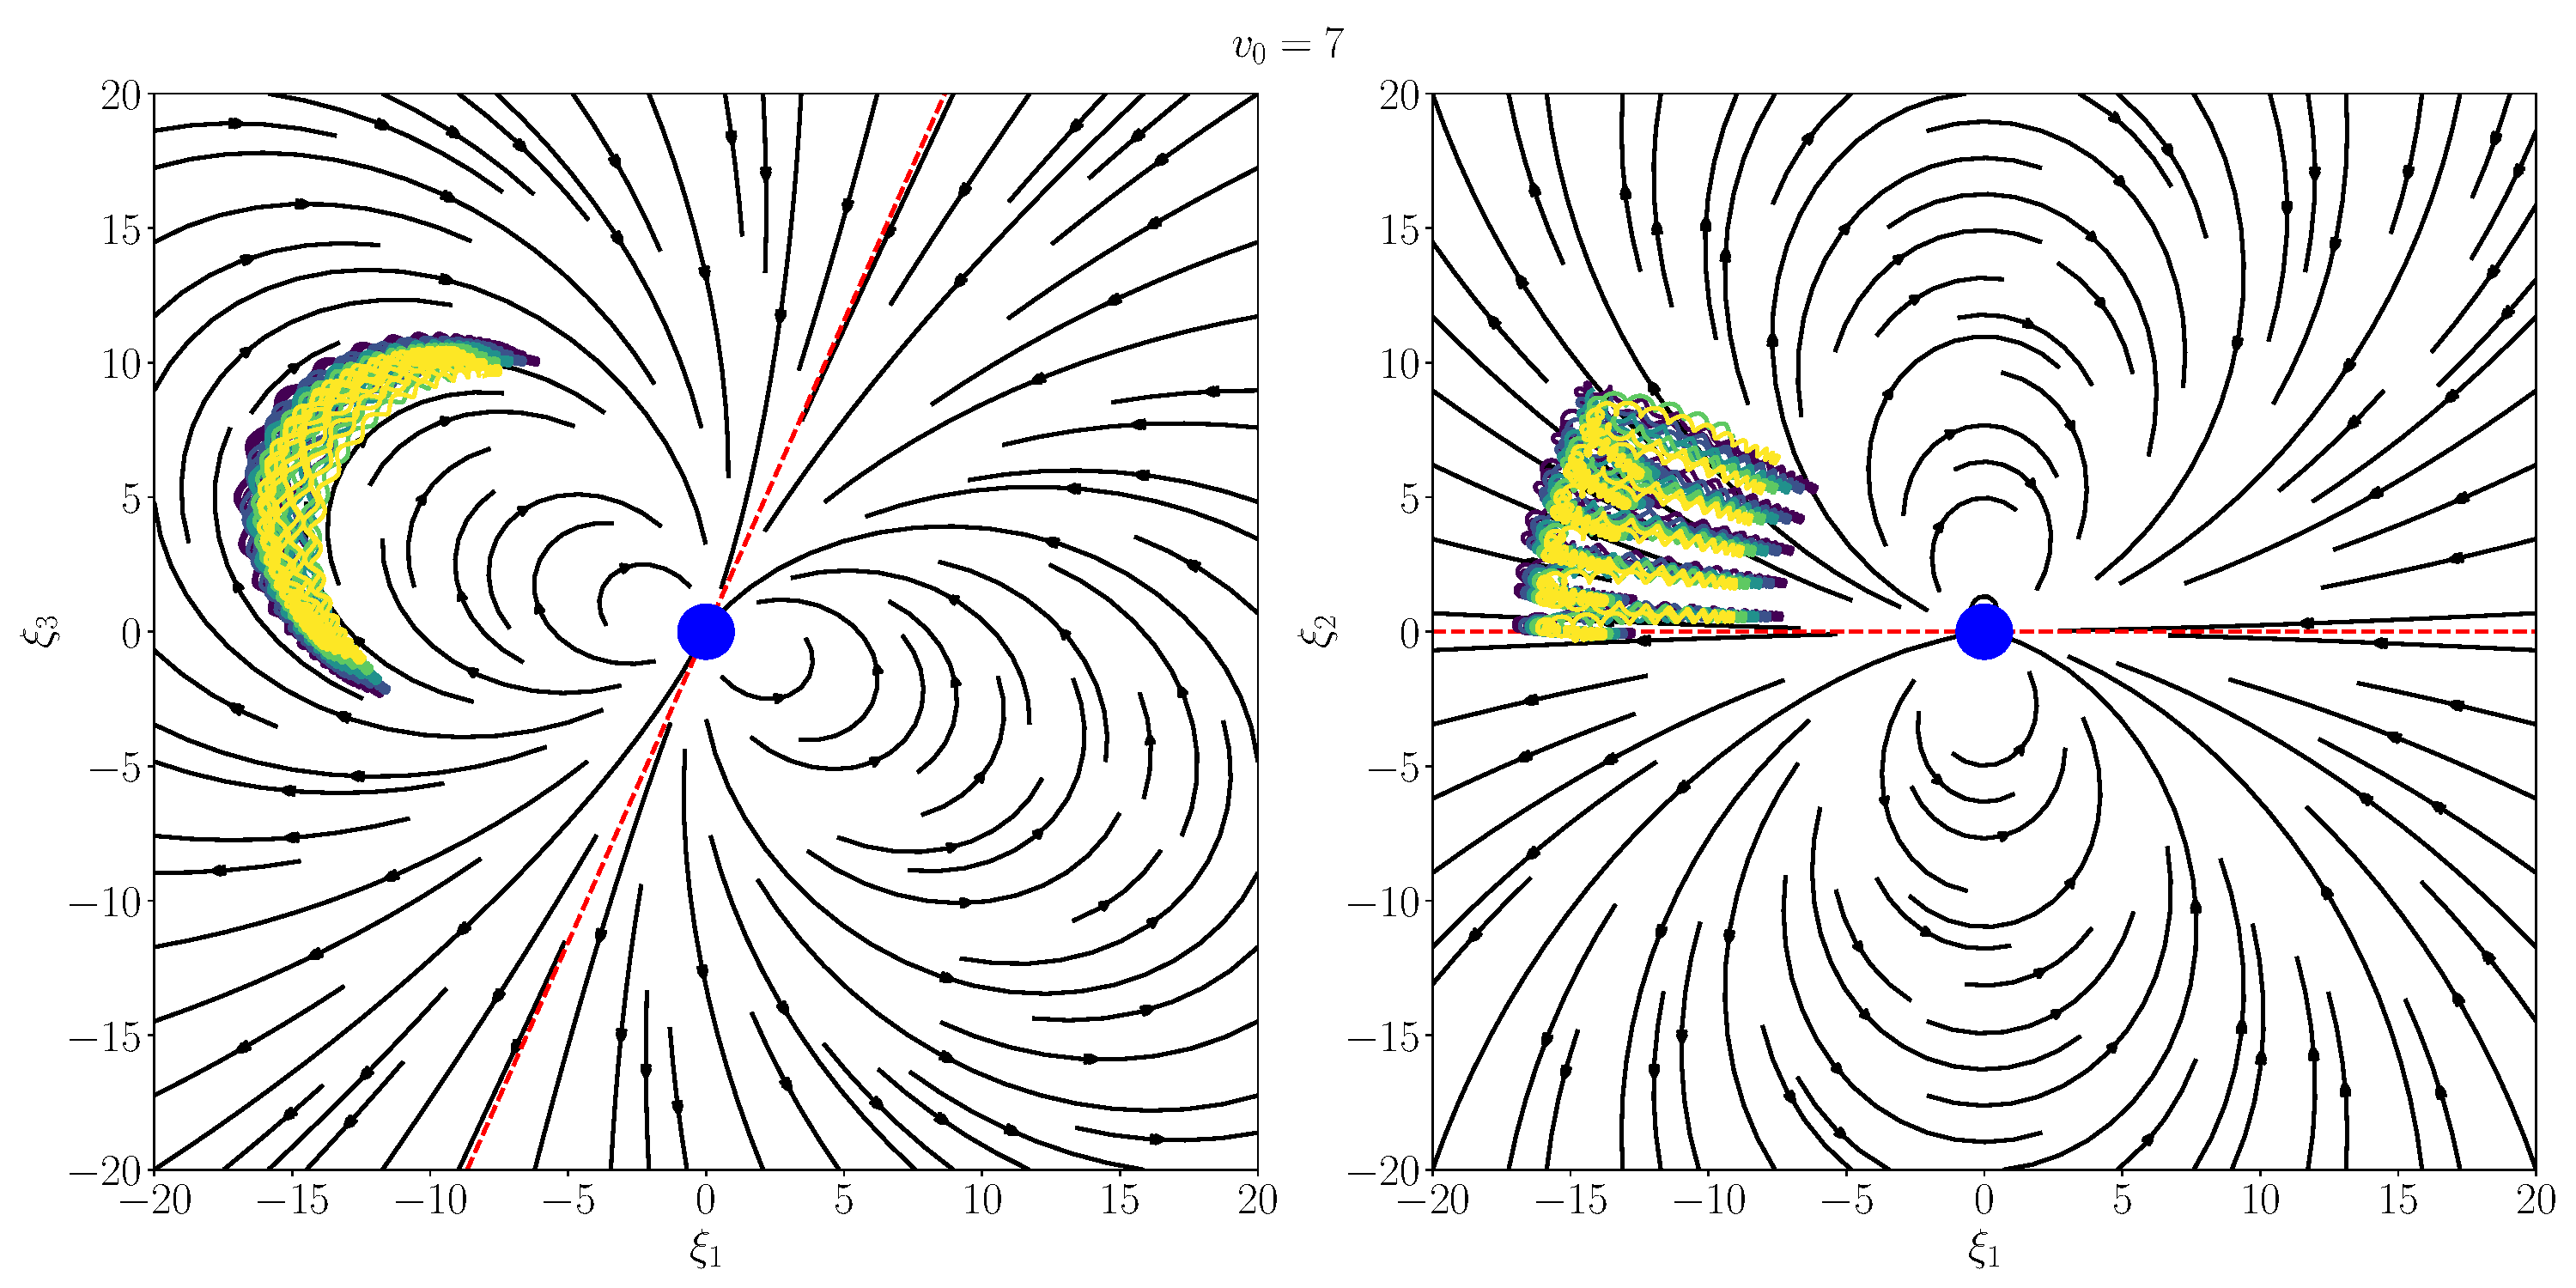
\includegraphics[width=\columnwidth]{../fig/traj_diffz.pdf}
	\caption{Particle sent towards the earth with typical solar wind velocity, for different heights $z0$}
	\label{fig:different_z}
\end{figure}

When doing this exact same simulation but with a weaker field ($\hat{B} \to 1/100 \hat{B}$) we observe that the same qualitative behaviour is captured. Moreover, we see here that the particles spiral in towards the poles. This is exactly what causes the Aurora. As seen from equation \eqref{eq:eom}, scaling the field is equivalent to scaling the velocity by the reciprocal factor. Hence, the behaviour shown in \ref{fig:weak_different_z} should be due to the \textit{fast} charged particles impinging on earth's magnetic field. 

\begin{figure}[htb]
	\centering
	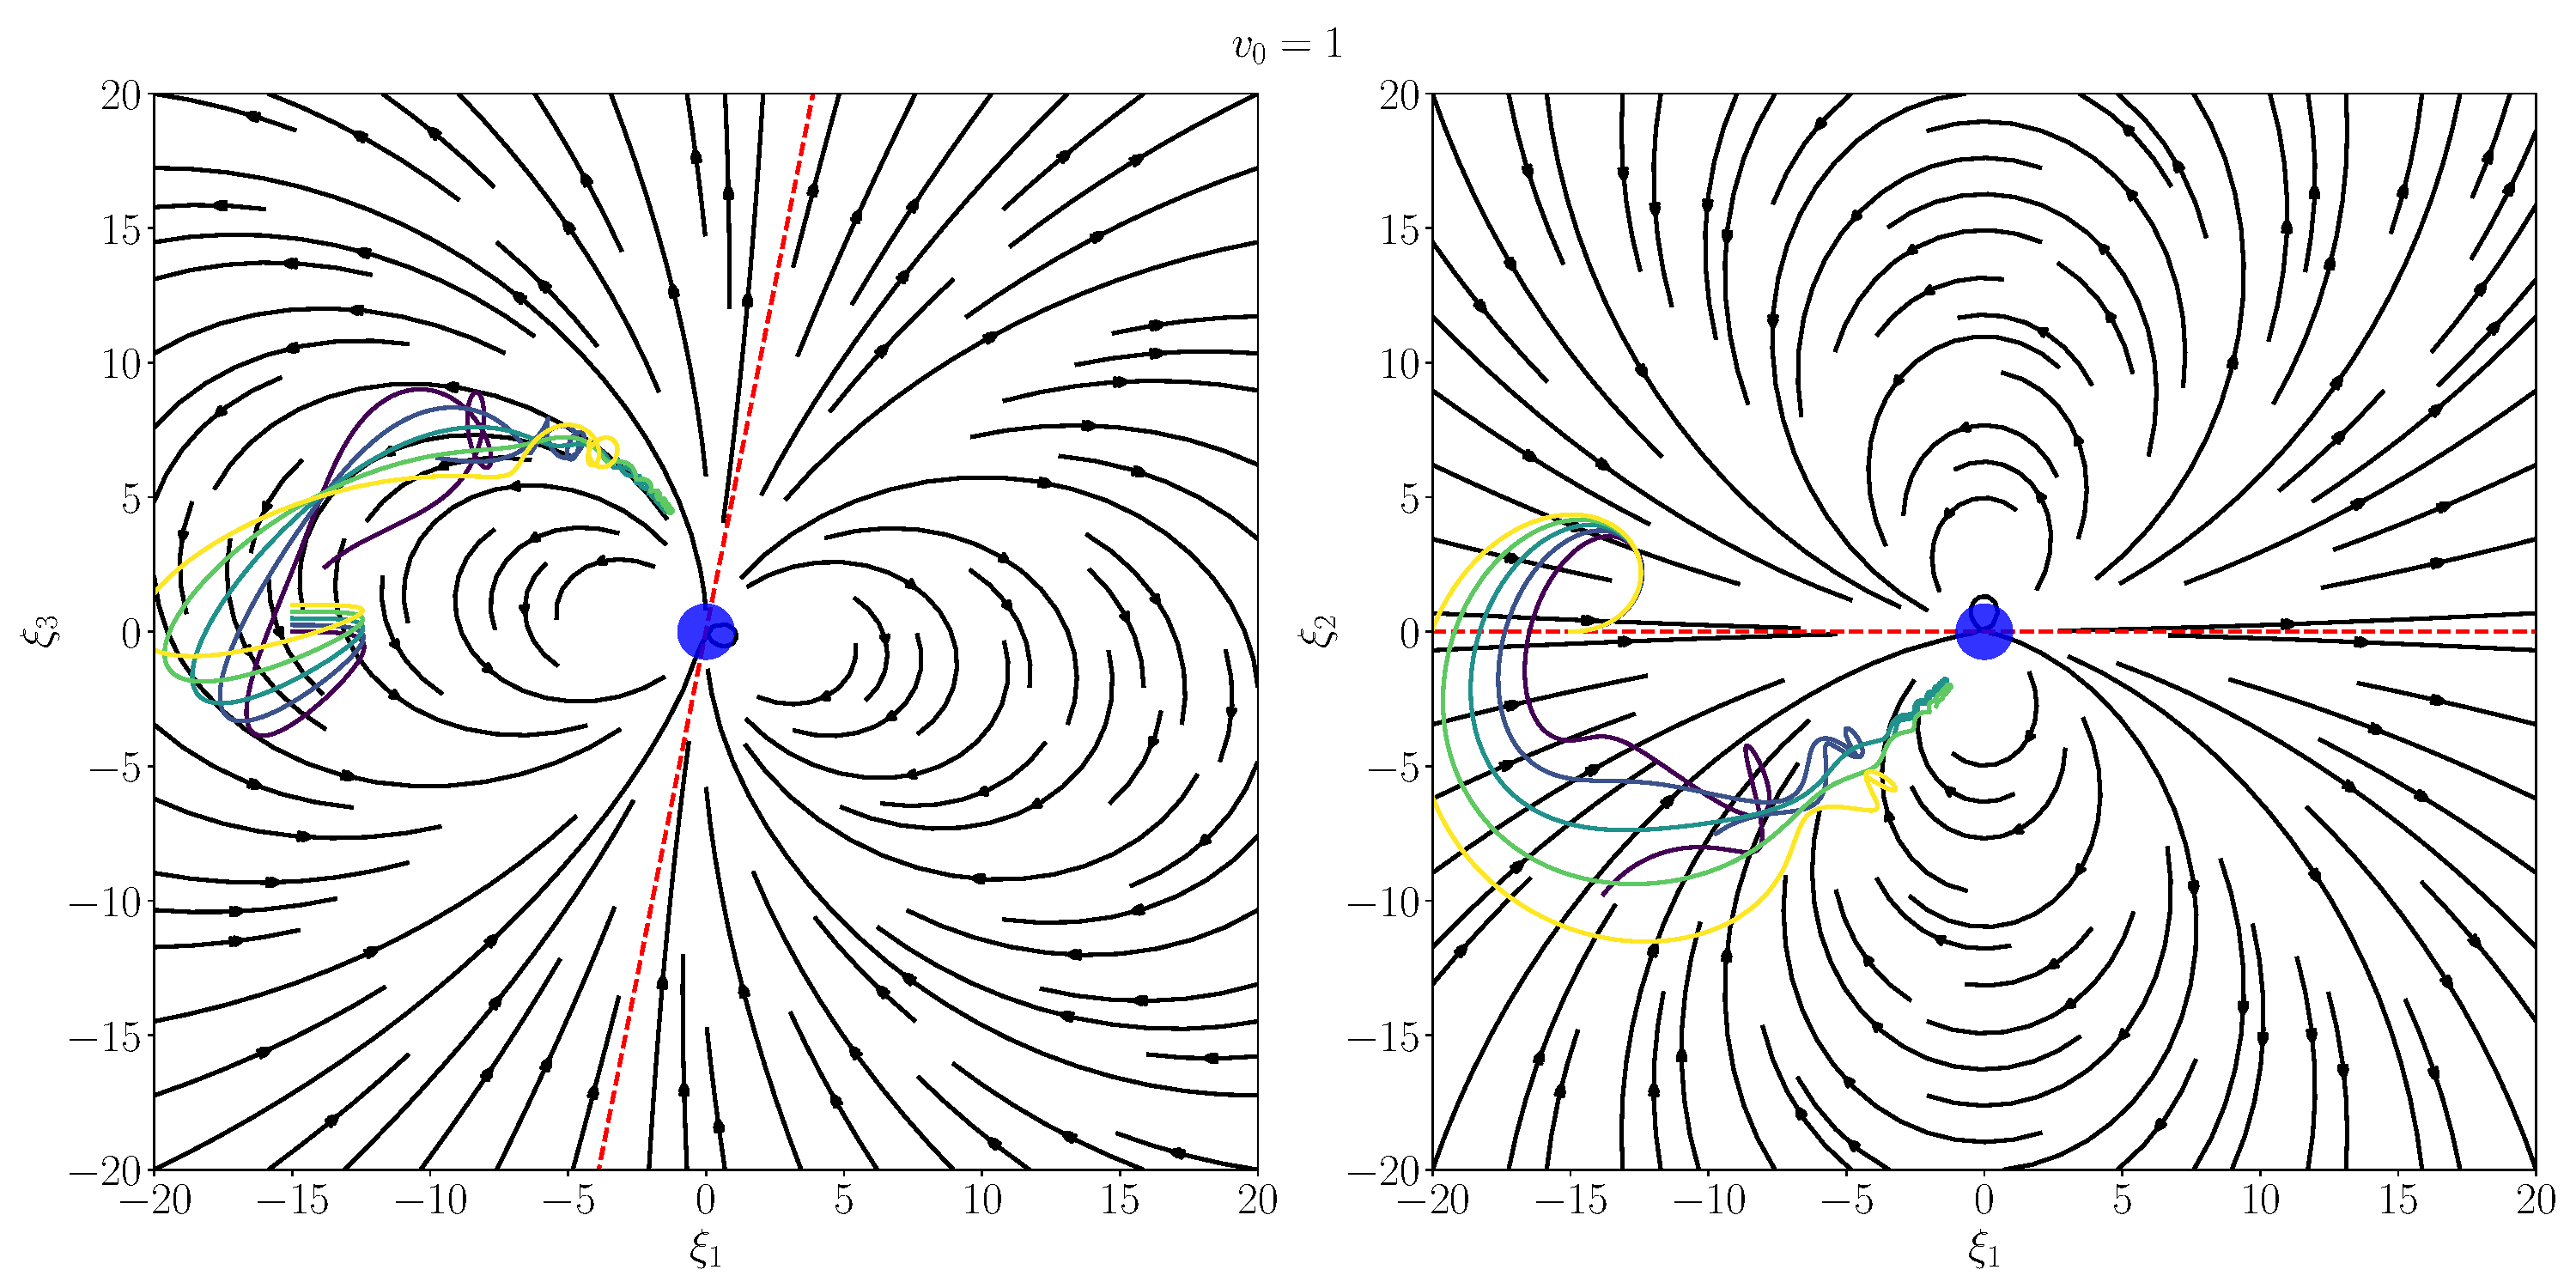
\includegraphics[width=\columnwidth]{../fig/strong_traj_diffz.pdf}
	\caption{Particle sent towards the earth with lower typical solar wind velocity, for different heights $z0$, with a weaker field.}
	\label{fig:weak_different_z}
\end{figure}

\subsection{Validity of solution}

To have an idea of how good the numerical solution is we investigate how well energy is conserved for the particles. Since magnetic forces do no work, the energy should be invariant. The (normalised) energy as a function of time is shown in figure \ref{fig:energy} for some of the paths plotted above.

\begin{figure}[htb]
	\centering
	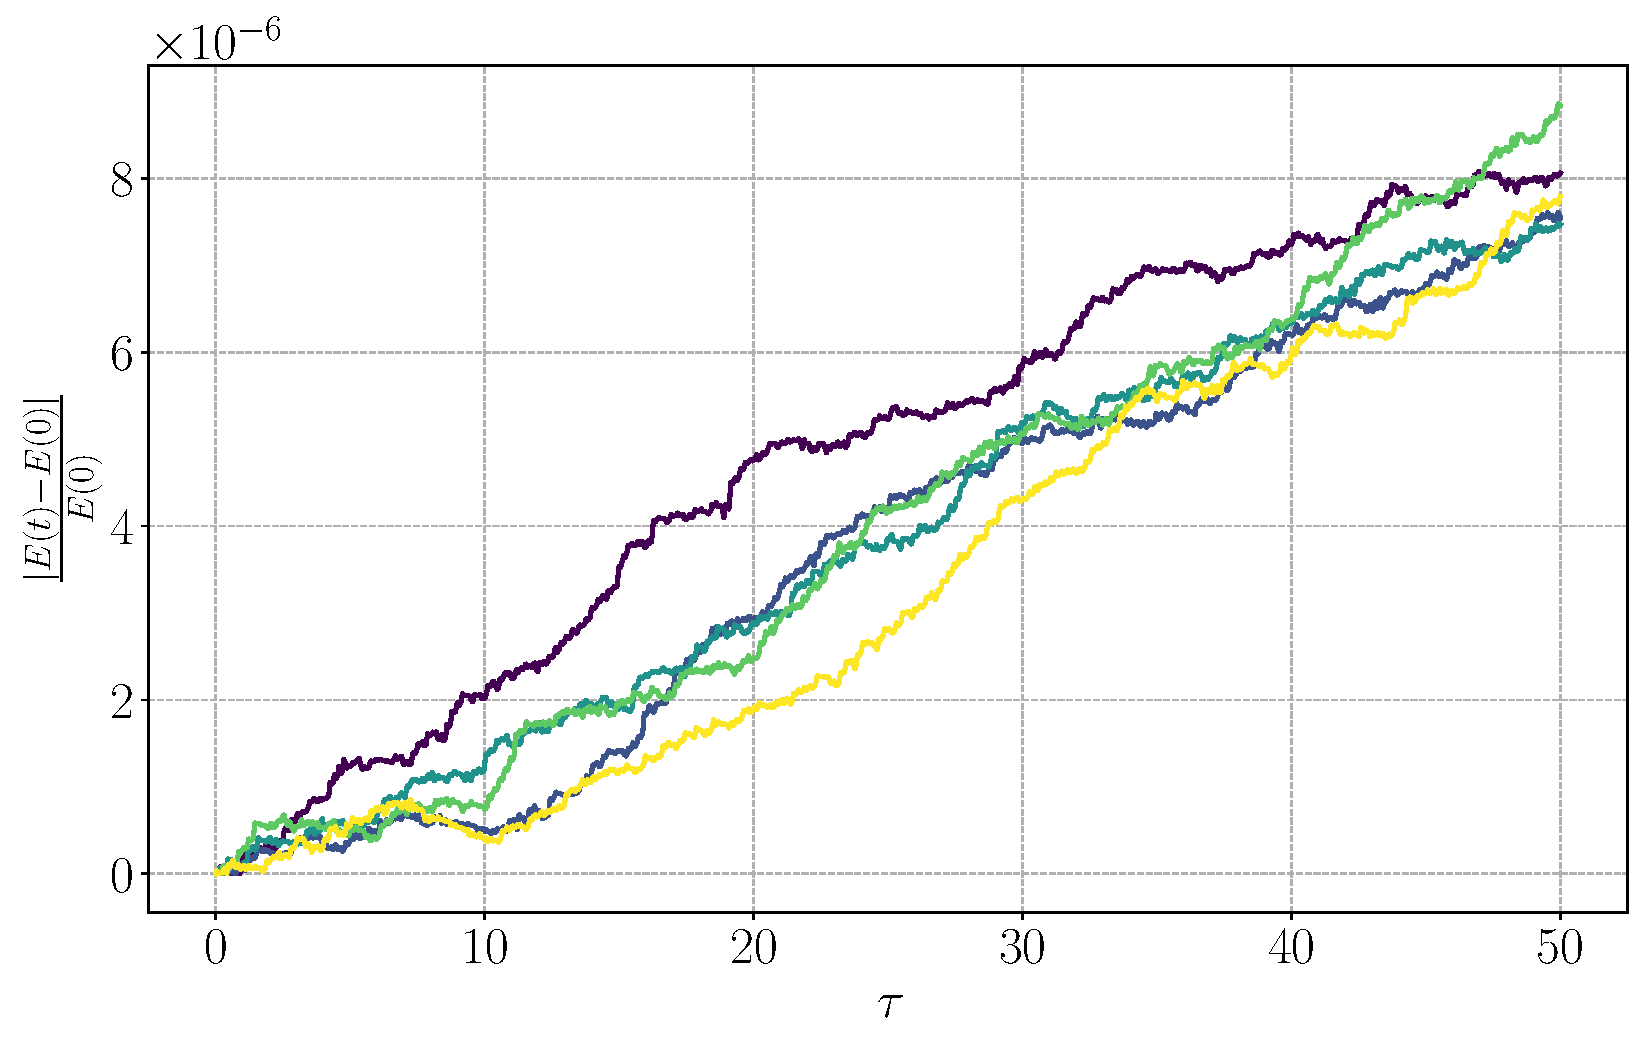
\includegraphics[width=0.8\columnwidth]{../fig/energy.pdf}
	\caption{Energy as a function of time for the $5$ trajectories shown in figure \ref{fig:different_z}.}
	\label{fig:energy}
\end{figure}

As the variations in the energy shown in figure \ref{fig:energy} are $\ll 1$ we conclude that the numerical validity of the solutions are good. There is however a slight drift in the energy, but that is inevitable when we take into consideration numerical round off errors. 
 